\chapter{The Death of Moore’s Law}\label{ch:3}
\section{Introduction}

The advent of RISC computing in the 1980s was the basis for Gordon Moore's initial prediction and faithfully showed a doubling in processor performance every 18 months. But, as the limits of clock frequency per chip began to appear, the use of Dennard scaling and multicore CPUs helped prolong the performance curve. But it is important to note that even at the start of the century, we were no longer on the Moore's Law curve, and doubling of performance took 3.5 years during this time. \\

Amdahl's Law refers to the limits of performance improvement that can be achieved with parallel processing. While parallelizing the execution of a process can provide an initial performance boost, there will always be a natural limit, as there are some execution tasks that cannot be parallelized. We have recently experienced that these limits come into effect when the benefits of using multiple CPU cores decrease, leading to an even longer time span between performance improvements. \\
The prediction, as can be seen in the graph, is that it will now take 20 years for CPU processing power to double in performance. Hence, Moore's Law is dead. \\

\pagebreak

\begin{figure}[h]
    \centering
    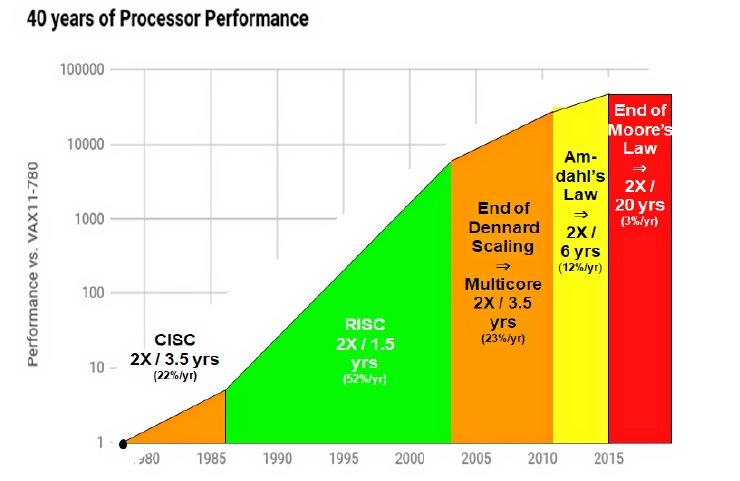
\includegraphics[scale=0.7]{figures/processor-performance.png}
    \caption{Source: John Hennessy and David Patterson, Computer Architecture: A Quantitative Approach, 6/e. 2018}
    \label{fig:gp}
\end{figure}

However, the underlying business model assumption here is that as the number of clients and volume of work increases, it is enough to simply add more servers. But, as can be clearly seen in the earlier graph, server processing performance will only grow 3\% per year over the next 20 years. This is far below the expectation that the amount of data to be processed will triple over the next five years
That's why the efficient use of that hardware is more important than ever and that requires the knowledge of algorithms and data structures. \\

\section{Algorithms in Big Tech Companies}
Most of the companies as a basis of their success used advanced algorithms to scale their service. One of the popular examples is Google, which used advanced web crawler technology and web site indexing to find information across the web. Google’s web crawler algorithm works in such a way, where it explores new sites existing on the web, based on visiting pre-existing site’s links, analyzing over 40,000 new pages in the web per second. After a page is crawled, Google tries to understand what the page is about. This stage is called indexing and it includes processing and analyzing the textual content and key content tags and attributes, such as <title> elements and alt attributes, images, videos, and more. All the process could be seen as a graph traversal procedure, where its page could be seen as a single node and links between pages could be viewed as edges. Using these technologies, they became a one of the significal companies in their field. \\

Another decent example could be Alibaba group, which used advanced algorithms in their cloud computing service in order to perform well on Single’s day, when the number of orders were at its peak. During this day Alibaba cloud processed 175,000 transactions and 120,000 per second at peak traffic, earning for a company around 84.54 billion U.S. dollars for two weeks according to 2021 yearly report. In order to perform well, they have used the Apache Flink framework, to distribute real time data across many clusters. However, to divide that data into meaningful chunks, they have used a sliding window algorithm, which is one of the most popular algorithms. Thus, the knowledge of good algorithms helped them to achieve their goal. \\

\begin{figure}[h]
    \centering
    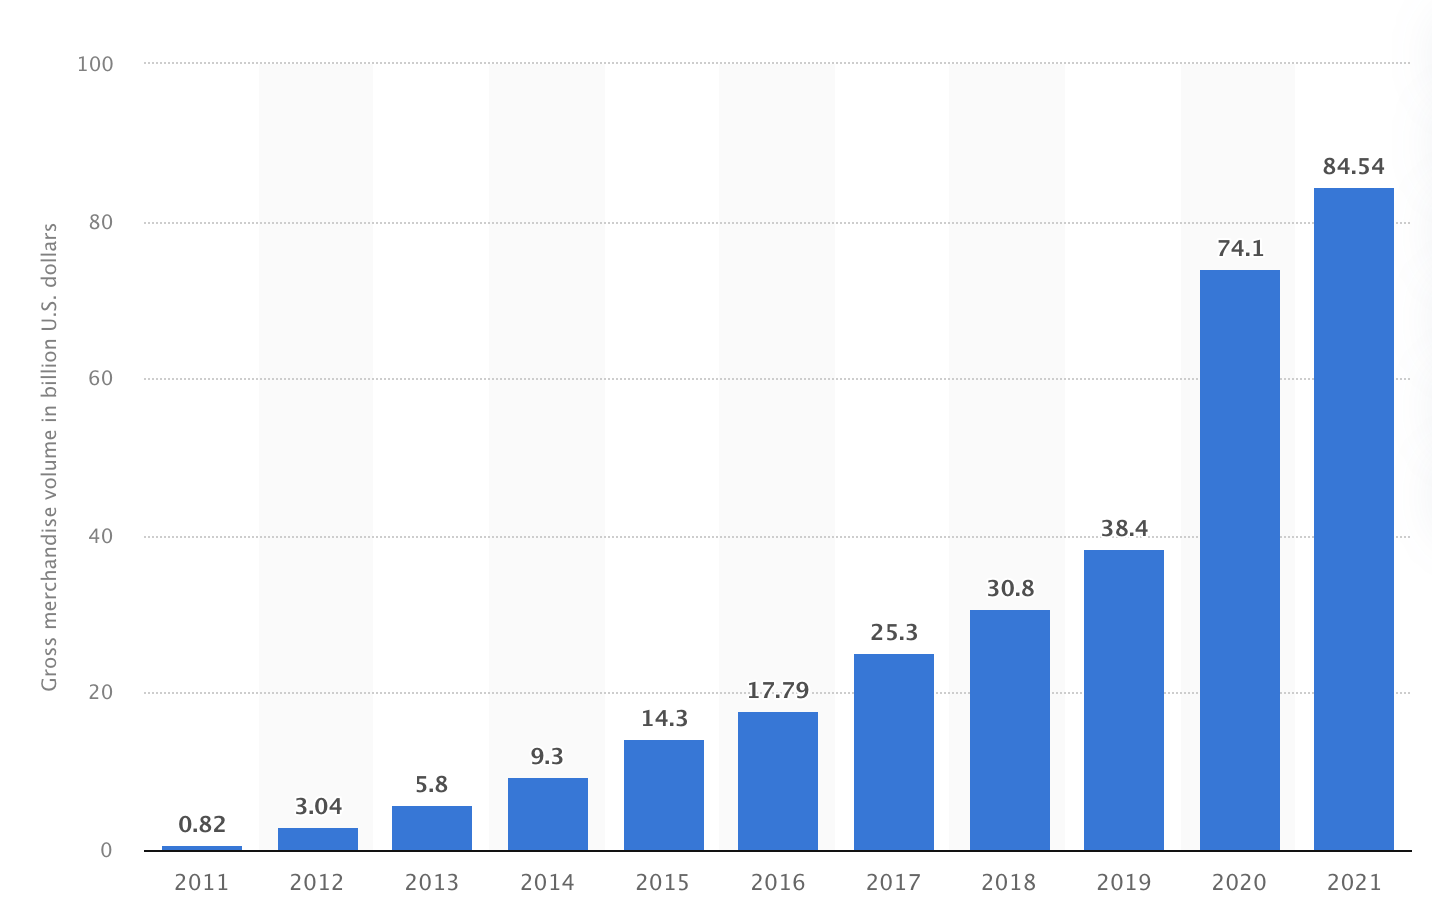
\includegraphics[scale=0.6]{figures/alibaba.png}
    \caption{Alibaba's gross merchandise volume on Singles' Day from 2011 to 2021 (in billion U.S. dollars)}
    \label{fig:gp}
\end{figure}

The other example could be Amazon, which incrementally updated the quality of their services in order to perform well on the market. At first, they only had e-commerce website with some goods, however to increase interest rate, they started to invent various algorithms, one of the examples is collaborative filtering algorithm, which was revolutionary 20 years ago. After a few years they have improved their algorithm adding some heuristics and by increasing computational power they made items on their site more customizable for a specific person, which greatly boosted the amount of their revenue in Amazon, Amazon Kindle and Amazon Prime. As for today, they use multilayered collaborative neural networks, to make the best possible predictions, which will be beneficial for their business.\\

Uber could be another good example, they use sophisticated path finding algorithms as Dijkstra and A star for cost and time optimization purposes. Using these algorithms at their core, they have created a good customer experience, which led to its becoming a multi-billion company.
